%!TEX root = /Users/andy/Documents/Academics/Dissertation/thesis.tex


\chapter{Neural activity of the Omega Turn}\label{chapter:omegaTurn}



\lettrine{R}{ecently, changes in the neural activity} of the  \textit{C. elegans}  motor circuit between  the worm's forward and reverse locomotion has been an area of intense study in laboratories around the world \citep{piggott_neural_2011, faumont_image-free_2011, kawano_imbalancing_2011, ben_arous_automated_2010}.
Three groups published work on this area in only the past few months \citep{piggott_neural_2011, faumont_image-free_2011, kawano_imbalancing_2011}. In the ongoing work presented here, we study the neural activity that underlies the omega turn, which also includes two such transitions between  forward and reverse locomotion. We confirm some of the results found by others and use our rich and detailed behavioral readout to probe more deeply at correlations between  neural activity and specific subtle behaviors critical for navigation. 

\section{Motivation}

Navigation is a goal directed locomotion, common across species, in which an organism moves toward or away from a cue.  At the neuronal level, navigation requires the temporal coordination of different motor programs.  How does an animal's nervous system orchestrate the changes in locomotion required for navigation? The \textit{Caenorhabditis elegans} escape response provides a platform upon which to investigate how navigation is carried out by a simple nervous system.  

Navigation in  \textit{C. elegans} is regulated by ventrally or dorsally biased head swings \citep{iino_parallel_2009} and deep ventral omega turns that reorient the worm in the opposite direction.  When the worm is touched on its anterior, it exhibits an escape response by pausing, reversing and turning ventrally in what is often called an omega turn.  The neural circuit for this escape response employs cells at all levels of the nervous system: mechanosensory neurons, command neurons, motor neurons, and muscle. The circuit plays an important role in the animal's decision making, the coordination of its motor programs and its turning behavior. 
The analysis of this stereotyped omega turn provides an opportunity to identify the  neuronal mechanisms that the nervous system employs to translate sensory information into navigational behavior.  


In this chapter we present ongoing work to explore the neural activity underlying the omega turn. A real-time tracking system was developed to record intracellular calcium transients in single neurons while simultaneously monitoring the macroscopic behavior of a freely moving worm as it undergoes an escape response.



 
\section{Dual-Magnification Calcium and Behavior Imaging}
\subsection{Background}
To study the neural activity of an omega turn requires a system that permits simultaneous observation of neural activity and behavior in freely moving worms.  In particular, it is important to be able to correlate individual neural activity to rich details of the worm's behavior, such as changes in curvature or direction.


Genetically encoded fluorescent calcium indicators such as Cameleon \citep{miyawaki_fluorescent_1997} and GCaMP \citep{tian_imaging_2009} are the primary tools available for optical neurophysiology in \textit{C. elegans}.  The fluorescence of these indicators change with the level of intracellular calcium present. Calcium is often a good indicator of neural activity. As a result, the fluorescent levels can be monitored and neural activity can be inferred.

Calcium imaging is often performed at high magnification (20x or more)  to resolve individual neurons and with high numerical aperture (NA) objectives to collect large numbers of photons. As a result, calcium imaging had traditionally been  performed on immobilized  \citep{clark_afd_2006} or partially restrained animals  \citep{faumont_awake_2006}, where it is possible to keep the neurons of interest in a small field of view for an extended period of time. 

The Samuel Lab pioneered the first system to perform calcium imaging in a moving worm \citep{clark_temporal_2007}. In that system, the user manually adjusted a joystick to track the neuron AFD in the head of an unrestrained worm on a motorized stage. The worm was imaged with a high NA 20x objective. This system allowed the user to observe calcium transients in a worm as it moved. Because the field of view only included a small portion of the worm,  details of the worm's behavior like its curvature were not visible.  Additionally, manual tracking made it difficult to consistently track abrupt changes in the worm's  motion.

Since then, a number of groups have developed manual \citep{kawano_imbalancing_2011} and automated \citep{faumont_image-free_2011, ben_arous_automated_2010, piggott_neural_2011} tracking systems for calcium imaging in moving worms, using either home built \citep{ben_arous_automated_2010, piggott_neural_2011,kawano_imbalancing_2011} or commercial \citep{faumont_image-free_2011} systems. These systems vary in the feedback rate, complexity, cost and in their ability to capture behavior data. For example, the systems presented in \citep{piggott_neural_2011} and  \citep{kawano_imbalancing_2011} lack the ability to view the entire worm in the field of view. 


We have a developed a new tracking system that offers unique advantages. The system is built around a spinning disk confocal microscope which cuts down on background fluorescence and increases signal to noise. The system identifies target neurons from the worm's outline, rather than from their fluorescence which makes it well suited for transgenic animals that exhibit fluorescence in more then one neuron. Most significantly, the system builds on previous experience developing rich behavioral monitors and thus provides high spatiotemporal behavioral data at 30 Hz including the worm's instantaneous curvature and orientation.  


\subsection{The DualMag System}

\begin{figure} %Schematic of DualMag
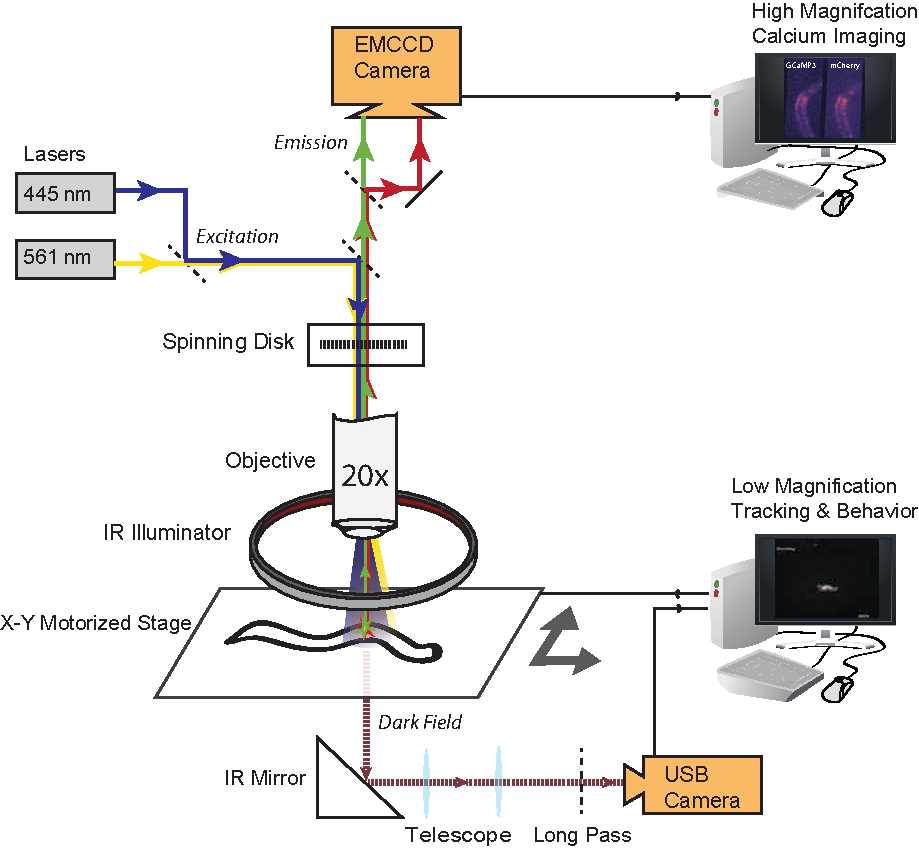
\includegraphics[width=\textwidth]{figures/omegaCalciumImagingSetup}
\caption[DualMag system apparatus.]{Schematic of the DualMag setup, permitting simultaneous recording of intracellular calcium transients and behavior in freely moving \textit{C. elegans}.  A transgenic worm, expressing GCaMP3 and mCherry in targeted neurons, crawls freely on a motorized stage under infrared illumination. An inexpensive USB camera images the worm's motion at low magnification. Real-time computer vision software rapidly analyzes each low magnification image and identifies the location and orientation of the worm and the targeted neuron and adjust the stage to keep the targeted neuron centered beneath a 20x objective used for calcium imaging.  Blue and yellow laser light shine through the 20x objective to excite GCaMp3 and mCherry in the targeted neuron. The emitted green and red fluorescence  is imaged through a spinning-disk confocal microscope onto two halves of an electron multiplying CCD camera.  Comparing the fluorescence in the green and red  channel images gives the relative level of calcium in the neuron. Slanted dashed lines indicate dichroic mirrors. \label{fig:omegaSchematic}}
\end{figure}



A tracking microscope was built capable of recording calcium transients in a moving worm. The microscope operates at two magnification levels simultaneously, one beam path operates at high-magnification to resolve single neurons, while the other beam path operates at low  magnification to view the entire body of the worm. Real-time computer vision software monitors the position of the body of the worm from the low-magnification beam path and adjusts a motorized stage to keep targeted neurons in the high-magnification field of view. The entire system is called the DualMag.


The DualMag system is built around an upright microscope body with a spinning disk confocal unit, a motorized stage and an additional low magnification imaging path. See Figure~\ref{fig:omegaSchematic} and Section \ref{sec:omegaOptics} for details.

A transgenic animal  expressing GCaMP3 and mCherry in targeted neurons crawls freely on agar in a petri dish on a motorized stage under dark field infrared illumination. The high magnification beam path illuminates targeted neurons with  blue (445 nm) and yellow (561 nm) laser light though the spinning-disk confocal system, emitting fluorescence from GCaMP3 in the green and from mCherry in the red. Dichroic mirrors filter out the excitation light and pass only the emitted light to a DualView unit which projects the red and green channels side-by-side onto the sensor of an  EMCCD camera. See Figure \ref{fig:omegaSampleImages}c and Section \ref{sec:omegaOptics}. 


\begin{figure}  %Sample Images of AVB 
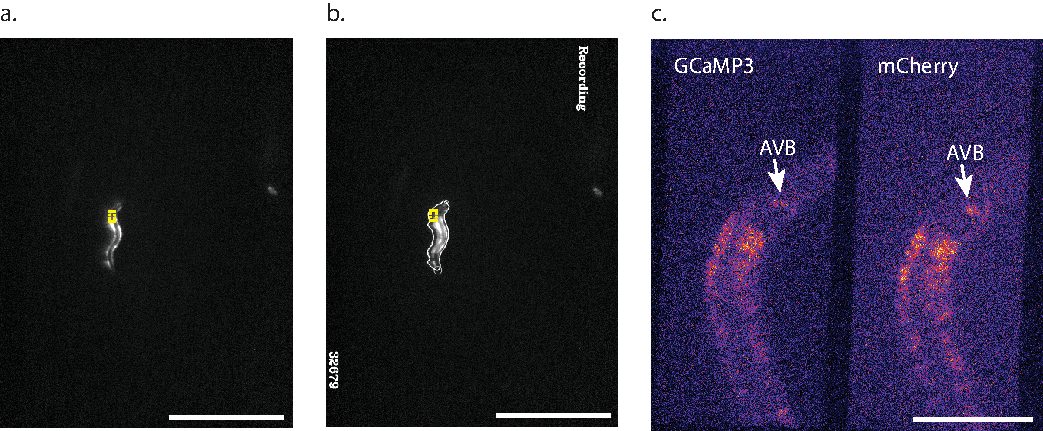
\includegraphics[width=\textwidth]{figures/omegaDualMagImagesWithScale}
\caption[Example images from the DualMag setup.]{Example images of the DualMag setup. Transgenic worm expressing GCaMP3 and mCherry in the AVB interneuron is observed in the DualMag system. \textbf{(a)} Raw-image of worm behavior recorded by the low-magnification beam path is shown. Scale bar is 1mm.  \textbf{(b)} Real-time computer vision software identifies the outline of the worm, its head and tail, and identifies the position of AVB for tracking. Scale bar is 1mm. \textbf{(c)} The high magnification beam path images the yellow square region shown in \textbf{b}. Green channel (left) shows calcium-dependent GCaMP3 fluorescence. Red channel (right) shows calcium-independent mCherry fluorescence. Scale bar is 100 \textmu m.
\label{fig:omegaSampleImages}}
\end{figure}

A second beam path, beneath the microscope images the infrared light scattered by the worm at low magnification. An inexpensive USB CCD camera monitors the worm's position and orientation at 30 fps. See Figure \ref{fig:omegaSampleImages}a. Custom real-time computer vision software written in C identifies the worm's outline, its head and tail,  and the location of targeted neurons (Figure \ref{fig:omegaSampleImages}b and Section \ref{sec:omegaSoftware}) and instructs the motorized stage to adjust its stage velocity to compensate for the worm's motion and to keep the targeted neuron squarely in the center of the high-magnification field of view. The feedback loop operates at 30 Hz and is sufficient to compensate for the worm's natural movements. See Figures \ref{fig:omegaTimeLapse} and \ref{fig:omegaMontage}.


\begin{figure}  %Time Lapse Image
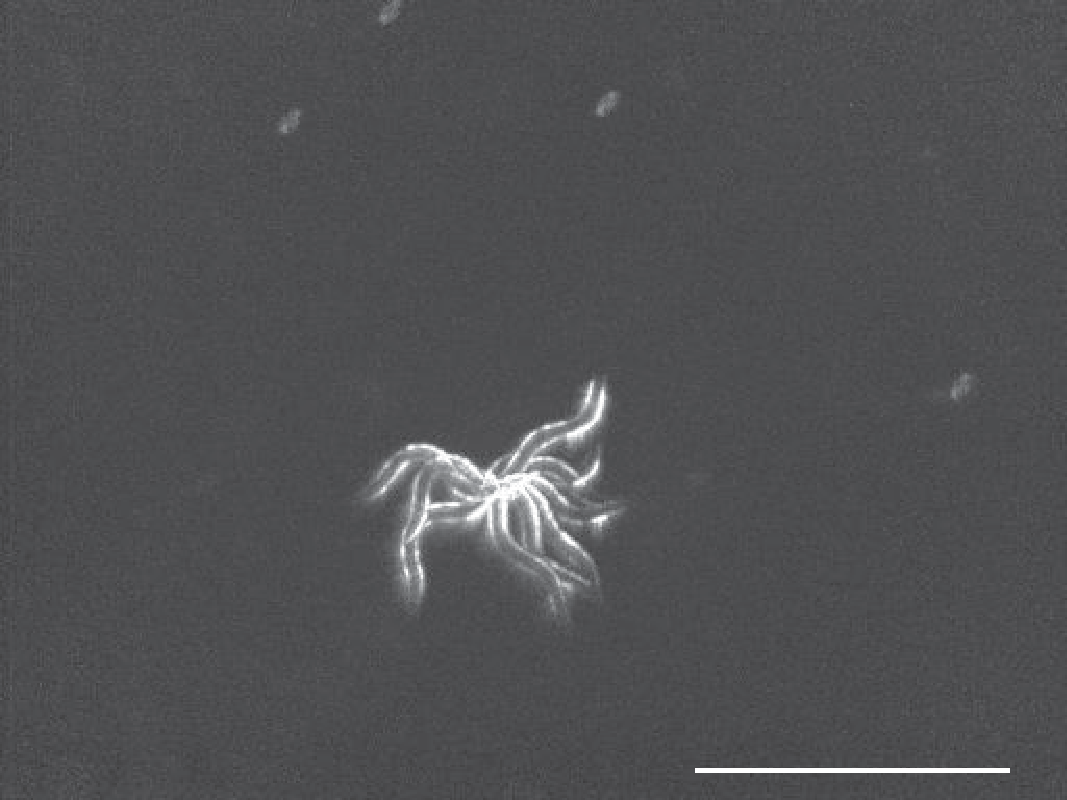
\includegraphics[width=\textwidth]{figures/omegaTimeLapse}
\caption[Time lapse image of behavior from low magnification beam path.]{Time-lapse stroboscopic darkfield image of worm behavior from the low magnification beam path is shown. The DualMag system continually adjusts the stage's velocity to isolate motion in a region of the worm's head. A 28 ms exposure image was taken every 3 seconds for 1 minute. Scale bar is 1 mm.
\label{fig:omegaTimeLapse}}
\end{figure}


While similar in principal to prior work \citep{ben_arous_automated_2010, piggott_neural_2011} this is the first system, to our knowledge, that uses a  spinning disk confocal microscope which cuts down on background fluorescence. Second, it uses an inexpensive USB camera to do the tracking and  leverages the real-time computer vision software from the CoLBeRT system \citep{leifer_optogenetic_2011} to perform rapid feedback based on the worm's morphology, not individual neuron fluorescence.





%HIstory: \citep{zheng_neuronal_1999}

\section{Neural Activity of the Escape Response}
The escape response in \textit{C. elegans} can be elicited by gently touching the anterior of the worm or by vibration. The response is  stereotyped: The worm first ceases its forward locomotion and exploratory head movements \citep{alkema_tyramine_2005}, it then moves backward away from the stimulus \citep{chalfie_neural_1985}, comes to a stop, and then bends its head ventrally to execute a deep ventral turn before finally reinitiating forward locomotion.  See Figure \ref{fig:omegaMontage}. The entire sequence is commonly referred to as an omega turn. 

\begin{figure}  %Montage of an Omega Turn
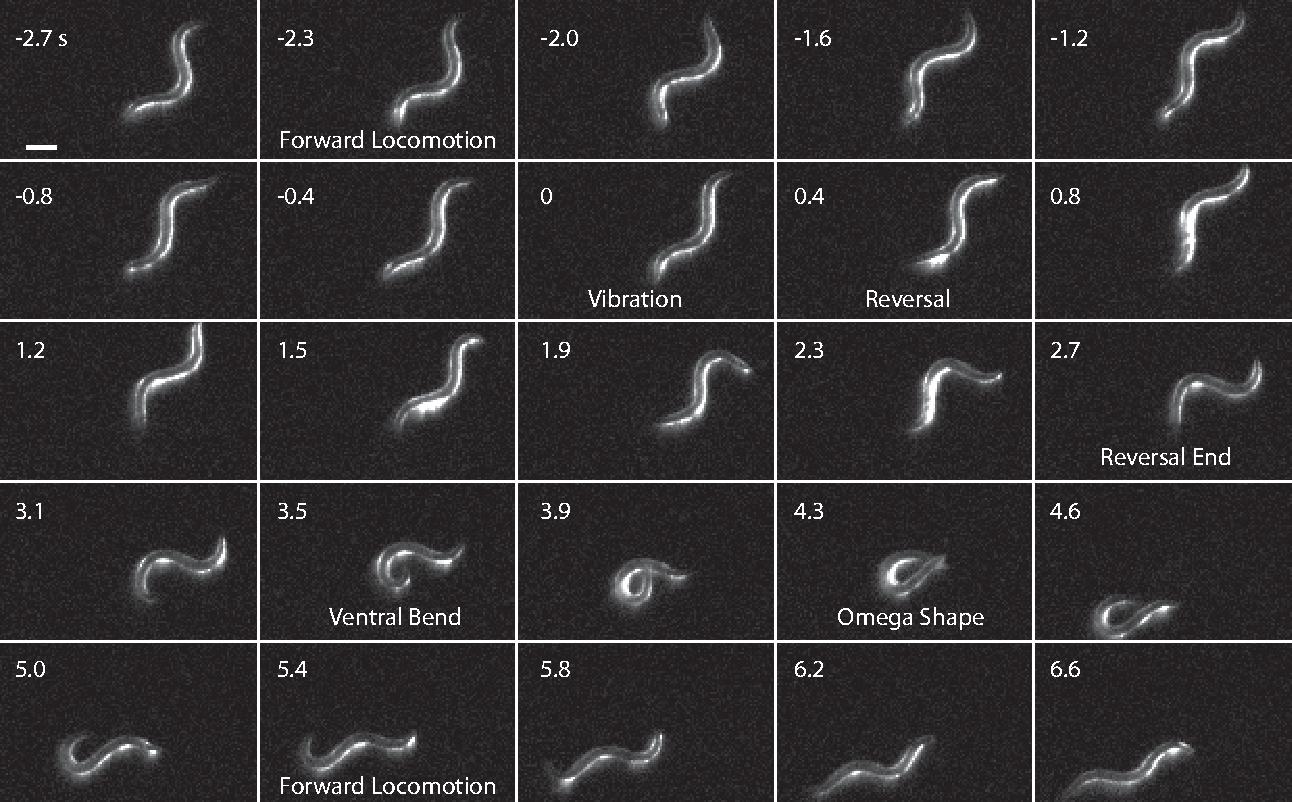
\includegraphics[width=\textwidth]{figures/omegaMontage}
\caption[Video of worm escape response.]{Video of worm escape response is shown. The worm undergoes forward locomotion.  At 0 s, an electric toothbrush vibrates the worm's petri dish and the worm halts forward locomotion and begins a reversal. At 2.7 s the worm ceases reversing and begins a deep ventral bend. At 4.3 s the worm exhibits the omega shape that gives the omega turn its name. At 5.4 s the worm recommences forward locomotion. Scale bar is 100 \textmu m.
\label{fig:omegaMontage}}
\end{figure}



 The escape response is initiated by mechanosensory neurons which transduce sensory information through locomotion command neurons to excitatory and inhibitory motor neurons that innervate the body wall muscles \citep{chalfie_neural_1985}. Laser ablation and genetic studies have  elucidated which neurons are required for which behavior \citep{chalfie_neural_1985, zheng_neuronal_1999, alkema_tyramine_2005}. A wiring diagram representing current thinking in the field is summarized in Figure \ref{fig:omegaCircuitDiagram}. Despite a rich literature describing which neurons are required for which behavior, it is only very recently that researchers have begun to study how neural activity correlates to behavior, and even then only in regards to forward versus backward locomotion \citep{piggott_neural_2011, faumont_image-free_2011, kawano_imbalancing_2011, ben_arous_automated_2010}. To fully understand the nervous system, one must also investigate the dynamics of neural activity and investigate the precise patterns and sequences of neural activity that drive behavior. As a first part of this ongoing work, the pattern of neural activity in the neurons AVA and AVB are investigated and correlated to the precise pattern of behavior exhibited by the worm during an omega turn. 

\begin{figure}  % Circuit Diagram
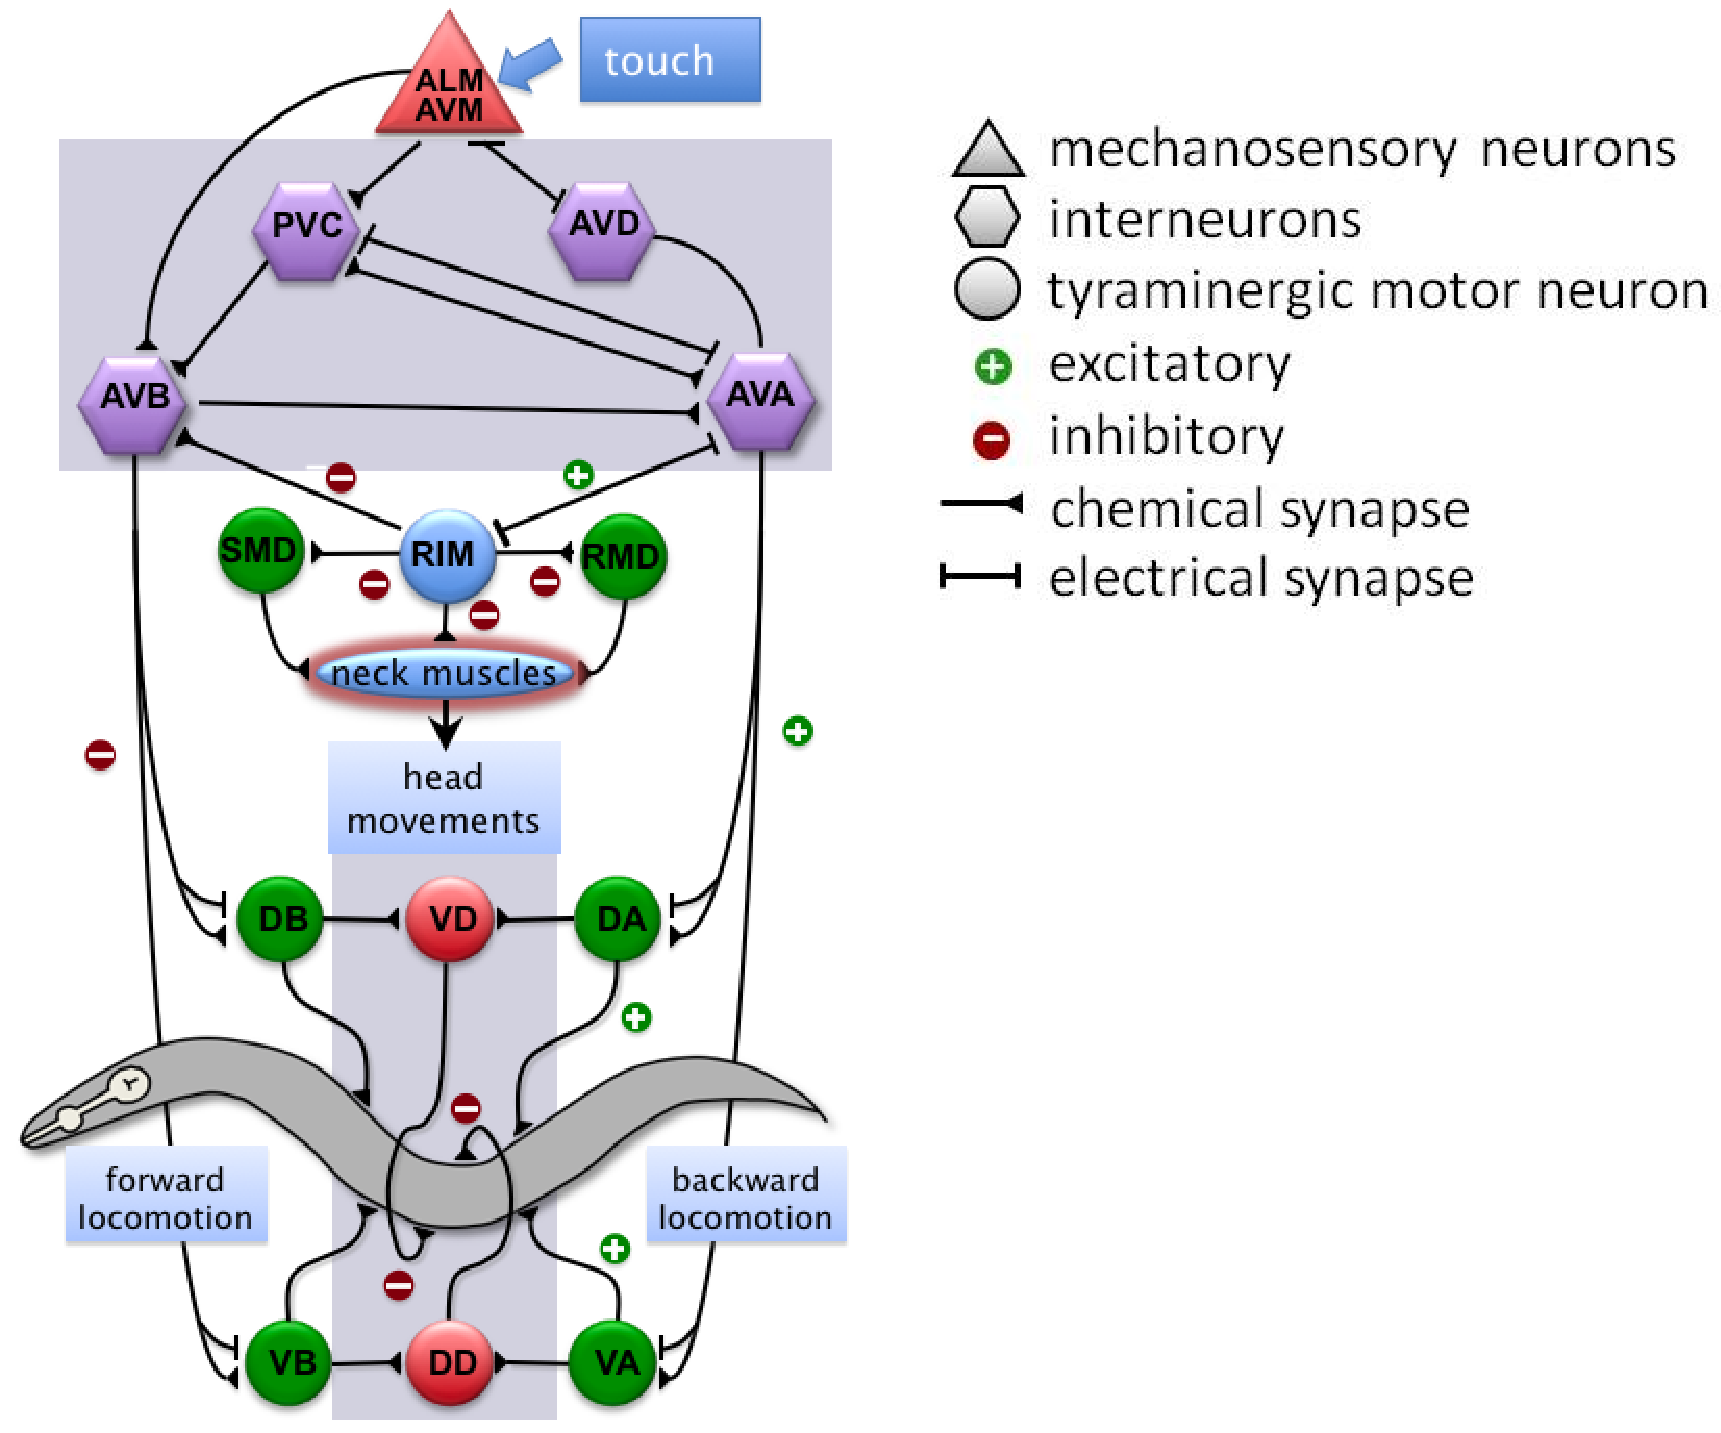
\includegraphics[width=\textwidth]{figures/omegaCircuitDiagram}
\caption[Circuit diagram representing current thinking in the field]{Circuit diagram showing neurons and their suspected role in the escape response. Information shown here is based on cumulative evidence from laser ablation and genetic studies performed by the community. Adapted from \citep{alkema_tyramine_2005} and \citep{pirri_tyramine-gated_2009}. 
\label{fig:omegaCircuitDiagram}}
\end{figure}

\section{Results}
\subsection{AVA}
AVA is a command interneuron involved in backward locomotion.  A P\textit{rig-3::mCherry::SL2::GCaMP3} transgenic worm, expressing mCherry and GCaMP3 in AVA is stimulated to undergo an escape response by transiently vibrating an electric toothbrush against the side of the agar plate containing the worm for less than half of a second.  As the worm freely crawls on the agar, its behavior and calcium transients are recorded. A representative sequence is shown in Figure \ref{fig:omegaAVArep}.  After vibration, calcium levels in AVA begin to rise as the worm reverses. The worm ceases backward locomotion, and undergoes a deep bend, visible as a large downward spike in the curvature diagram. Its body then forms a symmetric omega-like shape and the worm begins forward locomotion in a new direction, evident by the jump in  orientation. 


\begin{FPfigure}  %AVA representative results
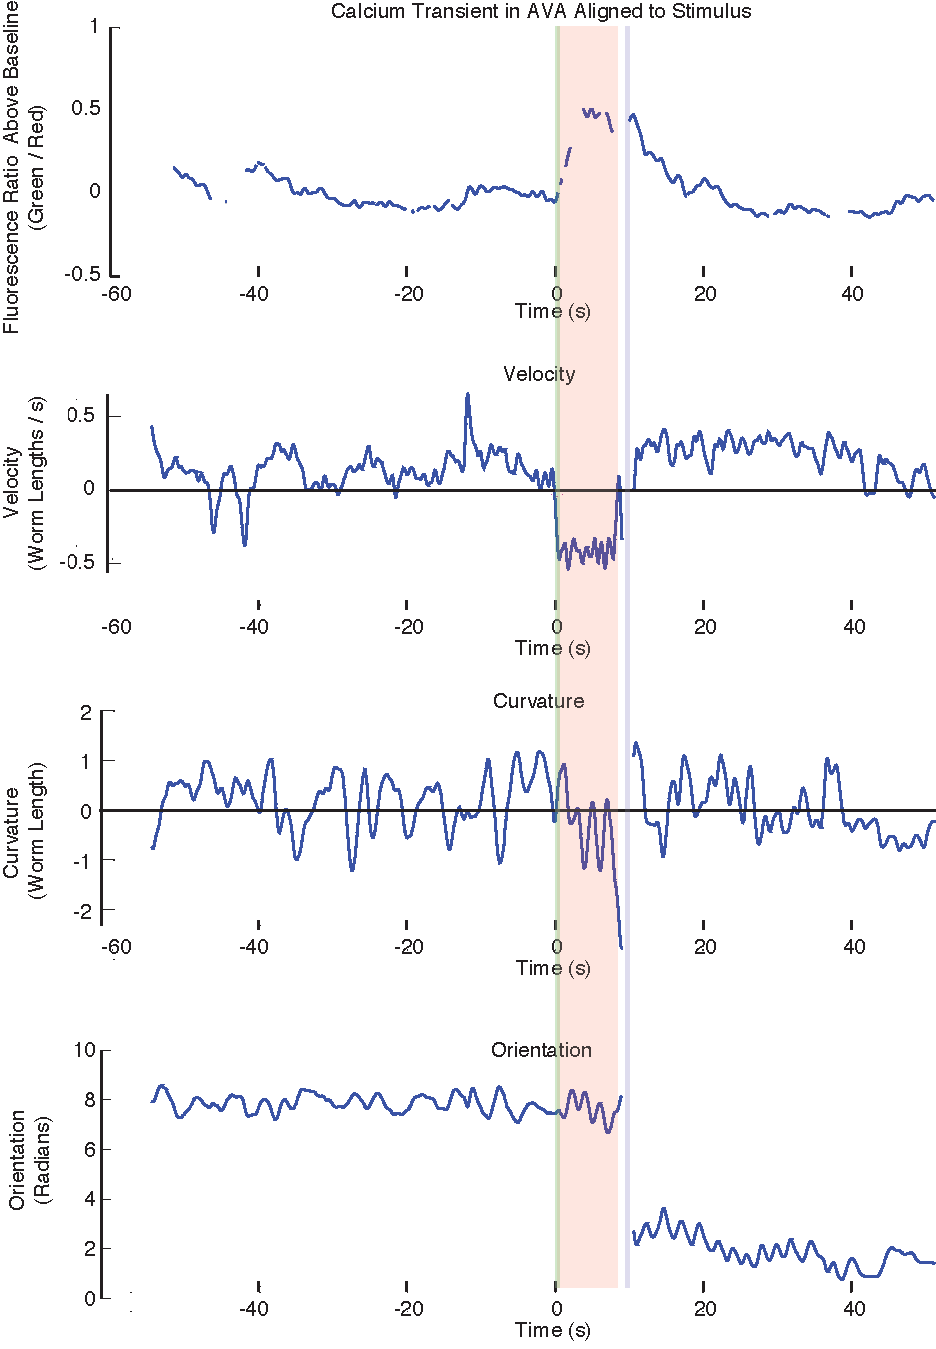
\includegraphics[width=\textwidth]{figures/omegaAVArep}
\caption[Neural activity of AVA and associated behavior.]{Calcium transient of AVA is shown with the worm's behavior.  A P\textit{rig-3::mCherry::SL2::GCaMP3} transgenic worm, expressing mCherry and GCaMP3 in its AVA interneuron is stimulated at time 0 s by vibrating its agar plate (light green background).  The worm ceases locomotion and reverses (light red background) and then forms an omega turn (light blue backround) before reinitiating forward locomotion. Changes in velocity, curvature and orientation corresponding to an omega turn are clearly evident.  Calcium levels in AVA increase as soon as the worm begins reversing and begin falling after re-initiation of forward locomotion. \label{fig:omegaAVArep}}
\end{FPfigure}


The fluorescence ratio is the ratio of the of intensities,  above background, of the pixels of AVA in the green to the red channel. Where presented, fluorescence ratio is plotted as the ratio above a baseline. The baseline is defined as the mean fluorescence ratio during a period from the beginning of a behavior sequence to the application of stimulus. Here, a behavior sequence is a defined as a region of behavior exhibiting only forward locomotion punctuated by exactly one omega turn in response to a stimuli. 

Where presented, velocity is the velocity of the worm's bending waves along its body, in units of worm length. Curvature is the curvature of the worm's centerline in a region 10 to 80 percent along its centerline from the anterior of the worm. A gap in the fluorescence trace indicates either an instance where the worm moves its head out of plane and the microscope transiently loses focus, or an instance when the tracking software incorrectly segments the worm and the neuron leaves the field of view.  A gap in behavior data reflects an instance when the software is unable to correctly identify the worm's head and tail, as occurs when the worm curls up in the omega shape. 


Neural activity and behavior have modest variation across trials and worms, but is overall stereotyped. The calcium transients in AVA of seven runs from four worms are shown in Figure \ref{fig:omegaAVA_aggregate}. The worm's velocity, curvature and orientation corresponding to these traces are shown in Figures \ref{fig:omegaAVA_velocity}, \ref{fig:omegaAVA_curvature} and \ref{fig:omegaAVA_orientation}, respectively. 




\begin{figure}  %AVA aggregated activity
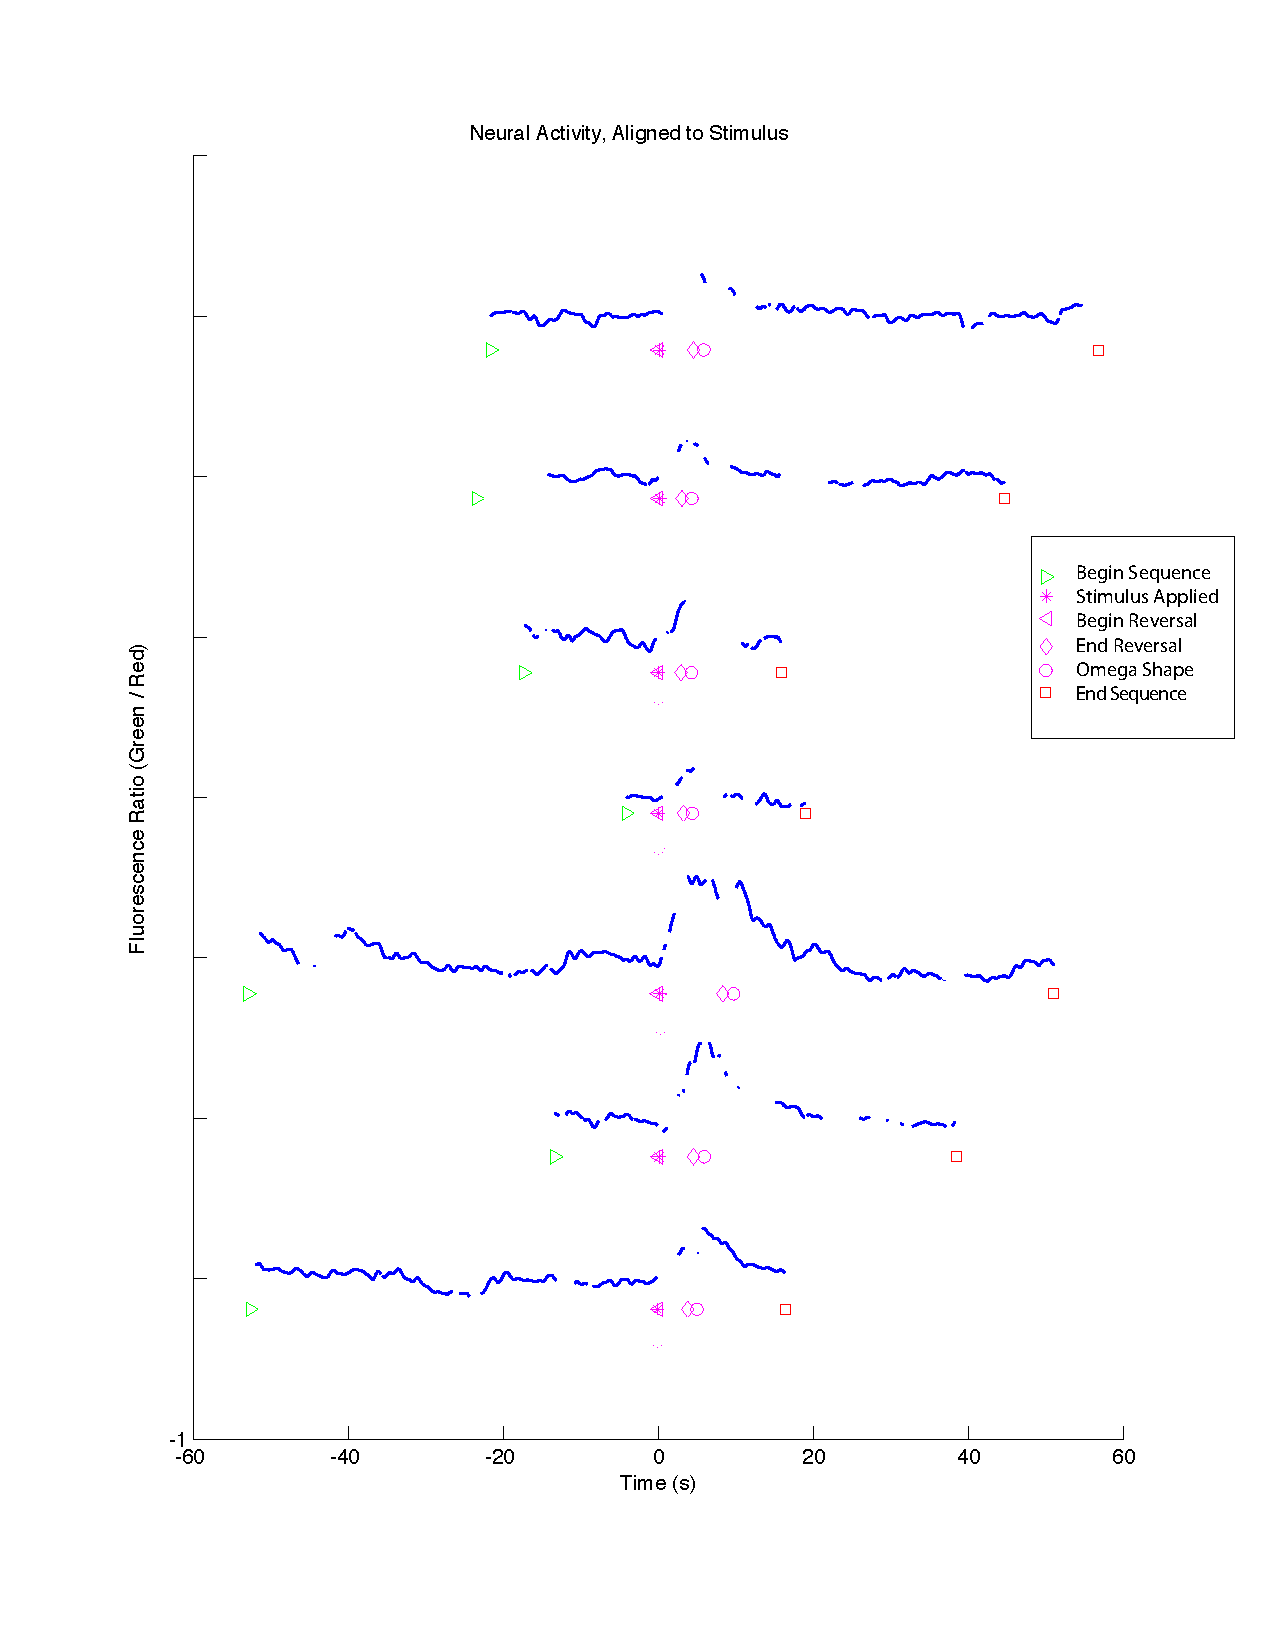
\includegraphics[width=\textwidth]{figures/omegaAVA_aggregate}
\caption[Neural activity of AVA for seven sequences from four worms.]{Calcium transients of AVA for seven behavior sequences from four worms.  A P\textit{rig-3::mCherry::SL2::GCaMP3} transgenic worm, expressing mCherry and GCaMP3 in its AVA interneuron, is stimulated at time 0 s by vibrating its agar plate. The fluorescence ratio is the ratio of the of intensities,  above background, of the pixels of AVA in the green to the red channel, plotted here as the ratio above baseline.  Corresponding velocity, curvature and orientation are shown in Figures \ref{fig:omegaAVA_velocity}, \ref{fig:omegaAVA_curvature} and \ref{fig:omegaAVA_orientation}, respectively. 
 \label{fig:omegaAVA_aggregate}}
\end{figure}



\begin{figure}  %AVA aggregated velocity
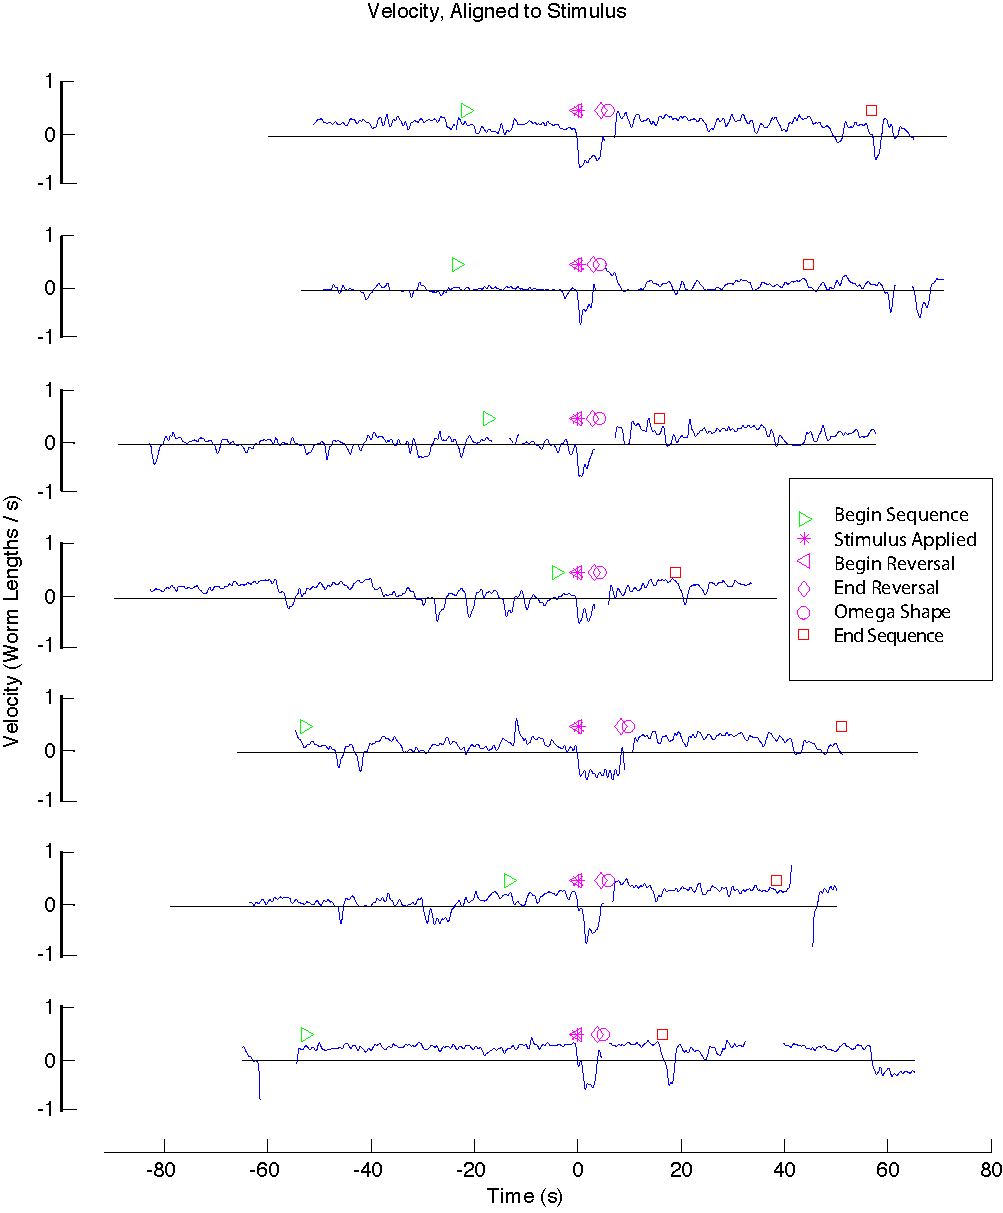
\includegraphics[width=\textwidth]{figures/omegaAVA_velocity}
\caption[Corresponding velocity for seven sequences from four worms.]{Velocity traces corresponding to AVA calcium traces shown in Figure \ref{fig:omegaAVA_aggregate}. A P\textit{rig-3::mCherry::SL2::GCaMP3} transgenic worm, is stimulated at time 0 s by vibrating its agar plate. Sustained negative dips correspond to reversals. Velocity, here, is the velocity at which the bending waves propagate along the worm's centerline.  The worm's corresponding curvature and orientation are shown in Figures \ref{fig:omegaAVA_curvature} and \ref{fig:omegaAVA_orientation}, respectively. \label{fig:omegaAVA_velocity}}
\end{figure}



\begin{figure}  %AVA aggregated curvature
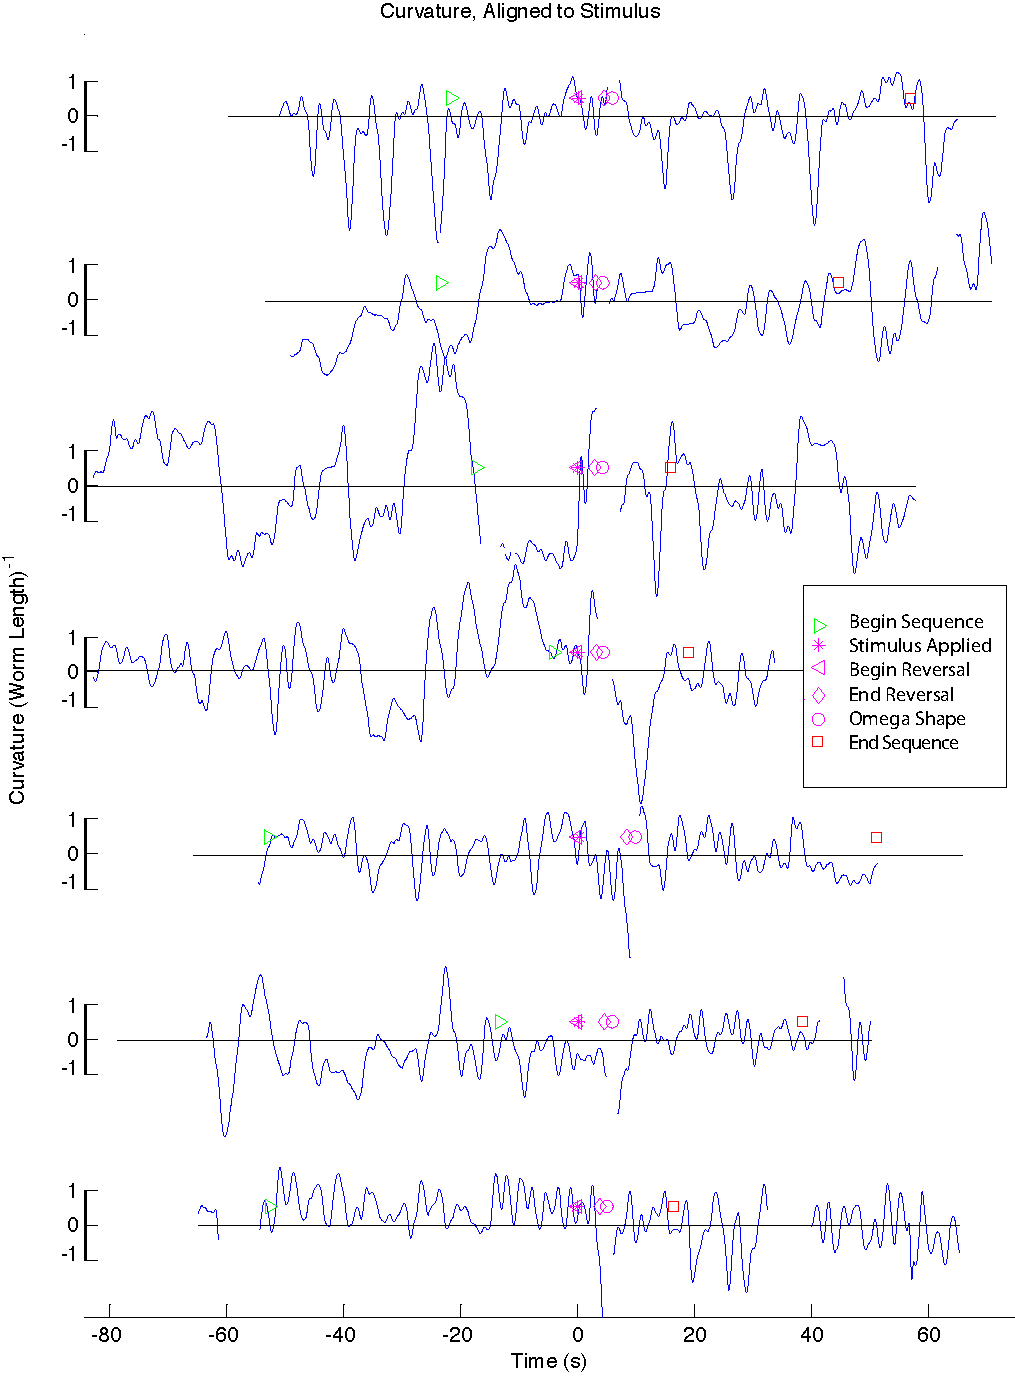
\includegraphics[width=\textwidth]{figures/omegaAVA_curvature}
\caption[Corresponding curvature for seven sequences from four worms.]{The worm's curvature ,corresponding to AVA calcium traces shown in Figure \ref{fig:omegaAVA_aggregate}. A P\textit{rig-3::mCherry::SL2::GCaMP3} transgenic worm is stimulated at time 0 s by vibrating its agar plate. A large spike or dip following the end of the worm's reversal (pink diamond) corresponds to a deep ventral bend. Here, curvature is the mean curvature of the worm's centerline in a region from 10\% to 80\% along its centerline. 
Velocity and orientation corresponding to these traces are shown in Figures \ref{fig:omegaAVA_velocity} and \ref{fig:omegaAVA_orientation}, respectively.  \label{fig:omegaAVA_curvature}}
\end{figure}


\begin{figure}  %AVA aggregated orientation
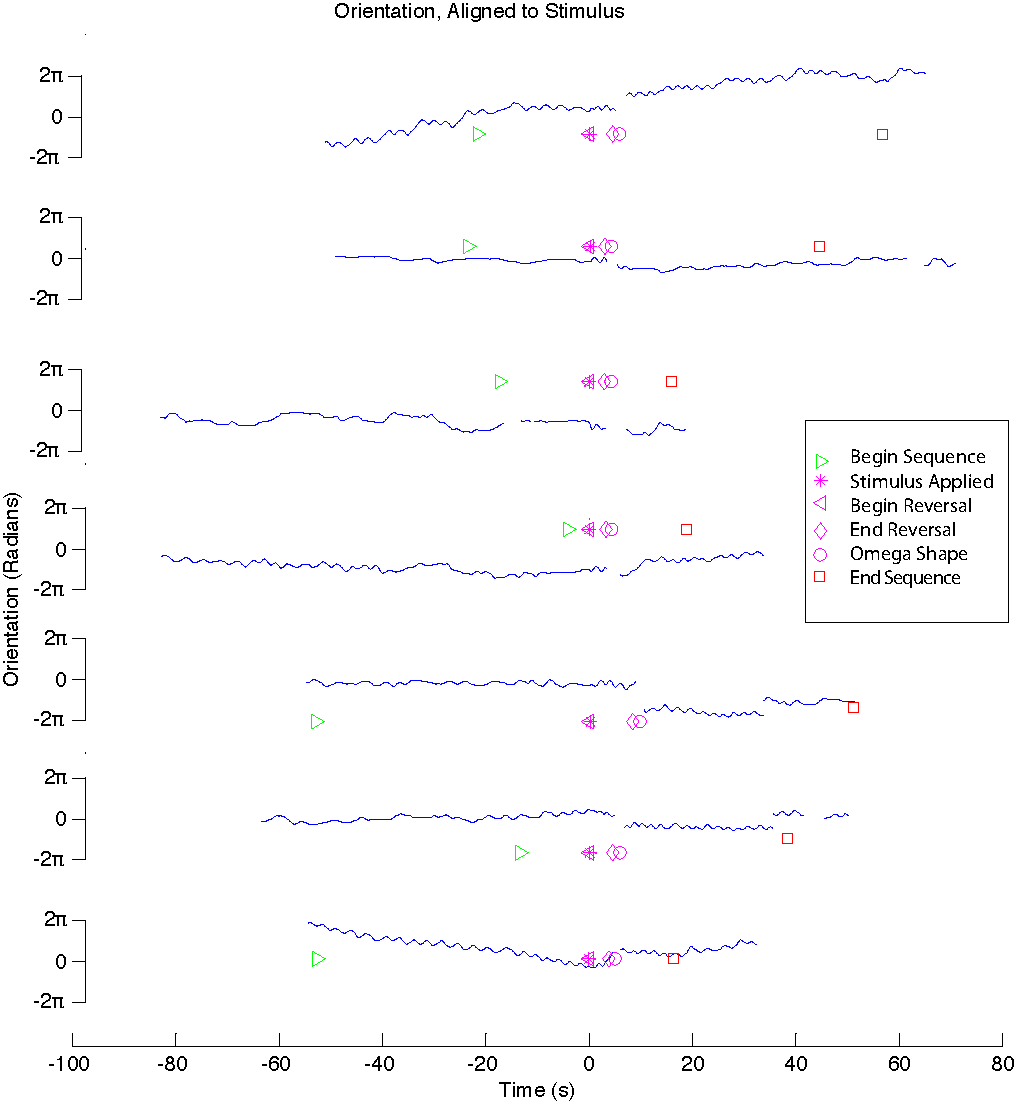
\includegraphics[width=\textwidth]{figures/omegaAVA_orientation}
\caption[Corresponding orientation for seven sequences from four worms.]{The worm's orientation, corresponding to AVA calcium traces shown in Figure \ref{fig:omegaAVA_aggregate}. A P\textit{lgc-55::mCherry::SL2::GCaMP3} transgenic worm is stimulated at time 0 s by vibrating its agar plate. A discontinuous jump around the time of omega-turn (pink circle) corresponds to an abrupt change in direction of motion. Here, orientation is the vector between the worm's neck and mid-region (5\%  and 40\%  along the from worm's centerlin anterior from its  head ). Velocity and curvature corresponding to these traces are shown in Figures \ref{fig:omegaAVA_velocity} and \ref{fig:omegaAVA_curvature}, respectively.  \label{fig:omegaAVA_orientation}}
\end{figure}

\subsection{AVB}
AVB is a command interneuron suspected to be involved in forward locomotion.  As with AVA above, a P\textit{lgc-55::mCherry::SL2::GCaMP3} transgenic worm expressing GCaMP3 and mCherry in the neuron AVB is stimulated by brief vibration. The worm undergoes an escape response and its calcium transients and behavior is measured.  See Figure \ref{fig:omegaAVBrep} for a representative trace.


\begin{FPfigure}  %AVB representative results
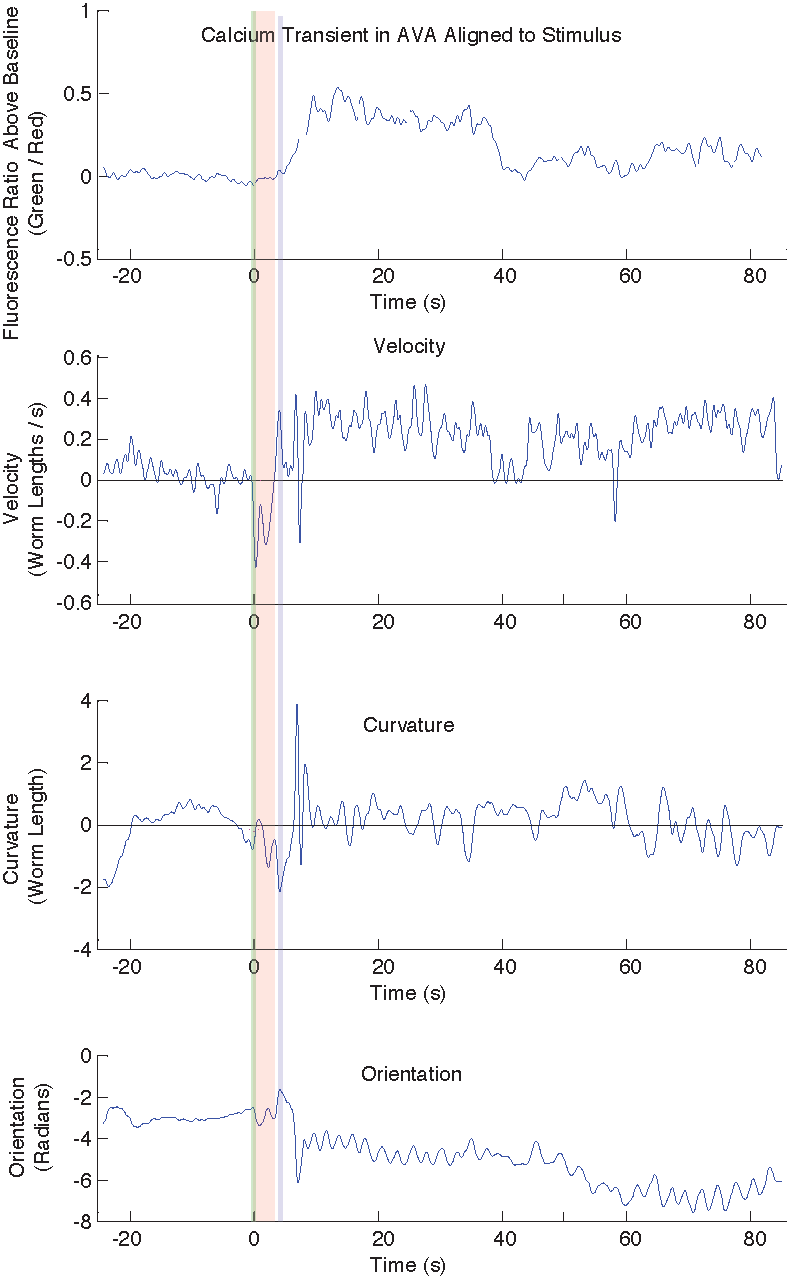
\includegraphics[width=\textwidth]{figures/omegaAVBrep}
\caption[Neural activity of AVB and associated behavior.]{Calcium transients indicating neural activity of AVB is shown with the worm's behavior.  A P\textit{lgc-55::mCherry::SL2::GCaMP3} transgenic worm, expressing mCherry and GCaMP3 in its AVA interneuron is stimulated at time 0 s by vibrating its agar plate (light green background).  The worm ceases locomotion and reverses (light red background) and then forms an omega turn (light blue backround) before reinitiating forward locomotion. Changes in velocity, curvature and orientation corresponding to an omega turn are clearly evident.  Calcium levels in AVA increase as soon as the worm begins reversing and begin falling after re-initiation of forward locomotion. \label{fig:omegaAVBrep}}
\end{FPfigure}




Prior reports \citep{zheng_neuronal_1999, kawano_imbalancing_2011}
 have suggested that AVB is active during forward locomotion. In our hands, AVB appears to become active after the worm completes the omega turn and begins forward locomotion. Preliminary results, however, suggest that AVB activity may turn off some length of time (\textasciitilde 30 seconds) after stimulus. Certainly in the trace shown here, AVB is inactive significantly before and after stimuli when the worm is undergoing forward locomotion. Perhaps AVB is involved in maintaining a sprint or some other sort of heightened state of activity immediately following reorientation.    More traces need to be recorded before any conclusions can be drawn.


\section{Discussion}	
Over a decade ago researchers used laser ablation studies to suggest the role that AVA and AVB might play in the motor circuit \citep{zheng_neuronal_1999}. This work confirms the results seen by others \citep{faumont_image-free_2011, ben_arous_automated_2010, piggott_neural_2011, kawano_imbalancing_2011} that AVA is active during reversals. This work also observes AVB activity. Preliminary results suggest that while AVB activity may be active with forward locomotion in response to a stimuli, it may not be persistently active during forward locomotion at all times. However, more recordings need to be performed to draw any conclusions. 

This ongoing work also provides a rich quantitative behavioral readout of the behavioral sequence of the escape response and omega turn. Features such as reversals, pauses, bends and reorientations can be precisely quantified by measuring the worm's velocity, curvature and orientation. When these metrics are recorded simultaneously with calcium transients, it then becomes possible to make correlations between neural activity and behavior. 

\section{Future}
This work is ongoing.  The instrumentation required to simultaneously monitor calcium activity and behavior is complete and has already been used to probe the command interneurons AVA and AVB, although more trials are needed. In addition to recording more traces from AVB, the authors are also in the process of observing the interneuron RIM, where there is currently controversy about the role it plays during a reversal.  

Eventually, this project aims to record calcium transients from all of the different neurons suspected to play a role in the escape response (Figure \ref{fig:omegaCircuitDiagram}) and explore their activity in relation to the worm's behavior.  The goal is to develop a picture of which neurons turn on and off when in the sequence of the escape response. Then a perturbative investigation can be performed, using tools like the CoLBeRT system (Chapter \ref{chapter:colbert}) to interrogate the individual contributions that silencing or stimulating each neuron gives to behavior. This will be a long-term project, but the groundwork has been laid here. 



\begin{comment}
Unraveling the neural circuitry required for turning behavior will lead to the understanding of the neural and molecular machinery that confers flexibility in the output of coordinated motor programs.
\end{comment}


\section{Methods}

\subsection{Strains}
The \textit{C. elegans} strains used include QW280: \textit{zfIs12[Prig-3::ChR2::GFP, lin-15(+)]}
, QW625: \textit{zfIs42[Prig-3::GCaMP3::SL2::mCherry; lin-15(+)]}, QW663: \textit{lin-15(n765ts); zfEx219[Pcex-1::GCaMP3::SL2::mCherry; lin-15(+)]}, QW666: \textit{lin-15(n765ts);
zfEx222[Plgc-55::mCherry::SL2::GCaMP3; lin-15(+)]}. Transgenic strains were
generated by microinjection of plasmid DNA along with the \textit{lin-15} rescuing construct
pL15EK into the germline of \textit{lin-15(n765ts)} mutants. ChR2, GCaMP3 and \textit{lin-
15(+)} plasmids were injected at 100 ng/\textmu l, 50 ng/\textmu l and 80 ng/\textmu l respectively.
Extrachromosomal arrays were integrated into the genome by X-ray irradiation (120kV)
for 10 minutes. Integrated strains were outcrossed four times to N2 wild type.

\subsection{Calcium Imaging in Moving Worm}
\subsubsection{Optics}\label{sec:omegaOptics}
A spinning disk confocal microscope built on a Nikon Eclpse LV 100 upright microscope frame  a foundation for the DualMag calcium imaging system. 

The spinning disk system is a CSU22 Confocal Scanning unit from Yokogawa that operates at 5000 rpm. Blue (445 nm) and yellow (561 nm) lasers are fiber-coupled into the spinning disk system. Lasers are housed in an  Andor Laser Combiner System 5000, and are controlled by an Andor Precision Control Unit 100 from Andor Technolgy. Confocal images are passed through a DV2 Dual-View  unit (MAG Biosystems) so that the red and green channel images are projected onto an an Andor iXon+ EMCCD camera under the control of Andor iQ 1.1.3 imaging software. Confocal images were captured at 20 fps with an exposure time of 50 ms. 

 A a 20x objective was used for an effective field of view, prior to the Dual-View, of about 300 \textmu m wide. At this magnification each laser  provided a maximum power of 20mW/mm$^2$ at the sample. In the experiments described here, the blue laser was run at 3 mW/mm$^2$ and the yellow laser was run at 10 mW/mm$^2$ to avoid pohotobleaching.

To image behavior, a custom made illumination ring of 100 850nm LED's was used to create dark field illumination by shining light  perpendicular to the main optical path. 

The condenser lens was removed from the bottom of the microscope to make room for a second low-magnifcation beam path to record the dark field imaging. An infrared prism mirror reflects infrared light into an optical train composed of a telescope and a 750nm long pass filter (Thorlabs, FEL0750).  An inexpensive USB CCD camera, DMK 31BUO3 from The Imaging Source,  was used to monitor the worm's behavior.  

The microscope stage was controlled by a Ludl Bioprecision2 XY motorized stage and MAC 6000 stage-controller. The worm was kept centered by a  feedback loop implemented by the real-time tracking software (see below).

\subsubsection{Real-Time Tracking} \label{sec:omegaSoftware}
Real-time tracking was performed by monitoring the image of the worm through the low-magnification dark field beam path and adjusting the velocity of a motorized stage. 1024 x 768 px grayscale images were acquiredfrom a USB camera 30 fps. A modified version of the MindControl software (Chapter \ref{chapter:coblert}) was used to track the worm and keep targeted neurons centered in the field of view of the high magnification beam path. In brief, the software identifies the outline of the worm, finds the head tail, segments the worm into coordinates, then identifies the targeted neuron within the coordinate system. Finally, the software measures the distance of the targeted neuron from the center of the high magnification field of view and adjusts the stage velocity to glide the worm back towards the center.

The software is essentially the same as in Chapter \ref{fig:colbert} with the following minor modifications, which were necessary to address poor lighting and the demands for more rapid tracking: When identifying the outline of the worm the software now performs a dilation on the image \citep{bradski_learning_2008} which can compensate for ``holes'' that appear in the worm due to lighting limitations. The newer version also allows the the outline of the worm to be smoothed directly, whereas the old version only allowed the underlying image be smoothed. Finally the new version of the software provides finer control of the stage response to the feedback loop. 

As before, the MindControl software was written in C using the OpenCV open source computer vision library \citep{bradski_learning_2008, bradski_opencv_2000} with the hardware optimized Intel Integrated Performance Primitives. 


\subsubsection{Video Synchronization}
The DualMag system records two independent video streams recorded at different frame rates on different computers. The two video streams are synchronized by shining synchronous pulses of LED light at the appropriate wavelength into both cameras. LEDs are controlled independently from the other software mentioned by a custom LabView program  interfaced with a LabJack U3-HV digital to analog converter. The flashes of light are identified manually during post processing. 

\subsubsection{Ratiometric Fluorescence Analysis}
Radiometric fluorescence analysis is performed offline in a quasi-manual process using custom scripts in MATLAB \citep{matlab_version_2010}.  The user selects control points to align the red and green channel images to each other. Scripts then prompt the user to manually click on the neuron of interest for every second frame of fluorescent imaging. The software searches in a local region nearby each mouse click to find the brightest pixel. A circular binary mask containing 50 pixels is drawn centered around the mouse click. This defines the region of interest containing the neuron.  The software interpolates to find the location of the neurons for the half of the frames that were not specified manually. For each frame, the software measure the mean intensity of the 20 brightest pixels in the region of interest in the red and green channels and subtracts off local background fluorescence. Background fluorescence is measured manually by finding the mean intensity of non-fluorescing regions of the worm in ImageJ \citep{rasband_image_1997}.

Fluorescent ratios are calculated as the ratio of the pixel intensities of the red and green regions of interest in each frame above background. When plotted, a baseline is subtracted from the fluorescent ratio.
 
Fluorescent images are recorded at 20 fps. Time-series traces of the fluorescent ratios were smoothed by linearly interpolating over any gaps and convolution with a Gaussian of $\sigma$=5 frames (\textasciitilde 250 ms) with padding of the end-point values. Finally points that had previously been interpolated were removed.


\subsubsection{Benavioral Analysis}
Behavior analysis was performed using a modified version of the MindControl Analysis scripts (Chapter \ref{chapter:colbert}), written in MATLAB \citep{matlab_version_2010}. Velocity is defined as before. in Chapter \ref{chapter:colbert}. Curvature here, is defined as the mean curvature of the worm's body as defined in Chapter \ref{chapter:colbert}, but averaged over the region of the worm's centerline from 10\%  to 80\% down from the anterior. Orientation is the arctangent of the vector defined by the points along the worm centerline 5\% and 40\% along the centerline from the anterior.


Time-series behavioral data was smoothed by linearly interpolating over any gaps and convolution with a Gaussian of $\sigma$=5 frames (\textasciitilde 170 ms) with padding of the end-point values. Finally points that had previously been interpolated were removed.



\section{Manuscript Information}
\subsection{Author Contributions}
The work presented here was done by Andrew M. Leifer in close collaboration with Christopher Clark and Mark Alkema of the Alkema Lab. Andrew Leifer built the hardware with Mason Klein. Christopher Clark and Andrew Leifer together performed all of the experiments. Christopher generated the worm strains. Andrew wrote all software and analyzed the data. Lauren Freeman built the video synchronization LED system. 

Both Andrew and Christopher wrote the manuscript. Mark Alkema contributed Figure \ref{fig:omegaCircuitDiagram}.




\begin{comment}

I will express the fluorescent calcium sensor, GCaMP3 (Tian et al., 2009), in the AVM and ALM mechanosensory neurons, the AVA and AVB locomotion command neurons; the RMD, SMD and RIV neck motor neurons; and muscles with the mec-4, rig-3, lgc-55, lim-4 and myo-3 promoters (Sagasti et al., 1999; Pirri et al., 2009; Brockie et al., 2001; Ardizzi and Epstein, 1987).  With these transgenic lines, I will analyze mechanosensory neuron, command neuron, motor neuron and neck muscle flourescence to determine their activity during turning behavior.

\end{comment}



\begin{comment}
Alkema, M.J., Hunter-Ensor M., Ringstad N. and Horvitz H.R. (2005). Tyramine functions independently of octopamine in the Caenorhabditis elegans nervous system. Neuron 46, 247- 260.

Ardizzi J.P. and Epstein, H.E. (1987). Immunochemical Localization of Myosin Heavy Chain Isoforms and Paramyosin in Developmentally and Structurally Diverse Muscle Cell Types of the Nematode Caenorhabditis elegans. Journal of Cell Biology 105, 2763-2770.

Brockie, P.J., Madsen, D.M., Zheng, Y., Mellem, J. and Maricq A.V. (2001). Differential expression of glutamate receptor subunits in the nervous system of Caenorhabditis elegans and their regulation by the homeodomain protein UNC-42. Journal of Neuroscience 21, 1510-1522.

Chalfie, M., Sulston, J.E., White, J.G., Southgate, E., Thomson, J.N. and Brenner, S. (1985). The Neural Circuit for Touch Sensitivity in Caenorhabditis elegans. Journal of Neuroscience 5, 956-964.

Gray, J.M., Hill, J.J. and Bargmann C.I. (2005). A circuit for navigation in Caenorhabditis elegans. Proceedings of the National Academy of Sciences of the USA 102, 3184-3191.

Iino, Y. and Yoshida, K. (2009). Parallel use of two behavioral mechanisms for chemotaxis in Caenorhabditis elegans. Journal of Neuroscience 29, 5370-5380.

Pirri, J.K., McPherson, A.D., Donnelly, J.L., Francis, M.M. and Alkema, M.J. (2009) A tyramine-gated chloride channel coordinates distinct motor programs of a Caenorhabditis elegans escape
response. Neuron 62, 526-538.

Sagasti, A., Hobert, O., Troemel, E.R., Ruvkun, G. and Bargmann, C.I. (1999). Alternative olfactory neuron fates are specified by the LIM homeobox gene lim-4. Genes \&  Development. 13, 1794- 1806.

Tian, L., Hires, S.A., Mao, T., Huber, D., Chiappe, M.E., Chalasani, S.H., Petreanu, L., Akerboom, J., McKinney, S.A., Schreiter, E.R., Bargmann, C.I., Jayaraman, V., Svoboda, K. and Looger, L.L. (2009). Imaging neural activity in worms, flies and mice with improved GCaMP calcium indicators. Nature Methods 6, 875-881.
\end{comment}
